\documentclass{resume} % Use the custom resume.cls style

\usepackage[left=0.4 in,top=0.5cm,right=0.4 in,bottom=0.3in]{geometry} % Document margins

\usepackage{graphicx}
\usepackage{fontawesome5}
\usepackage[absolute,overlay]{textpos}

\newcommand{\tab}[1]{\hspace{.2667\textwidth}\rlap{#1}}

\newcommand{\itab}[1]{\hspace{0em}\rlap{#1}}

\name{Sagi Amangeldi}
\address{Tokyo, Japan}
\address{{\bf  \faIcon{envelope}} {\href{mailto:cap.cafu@gmail.com}{\color{blue}{cap.cafu@gmail.com}}} \\ {\bf \faIcon{linkedin}} {\href{https://www.linkedin.com/in/sagiamangeldi/}{\color{blue}{sagiamangeldi}}} \\ {\bf \faIcon{github}} {\href{https://github.com/capCafu}{\color{blue}{capCafu}}}}

\begin{document}
\begin{textblock*}{3cm}(17.6cm,0.1cm)
    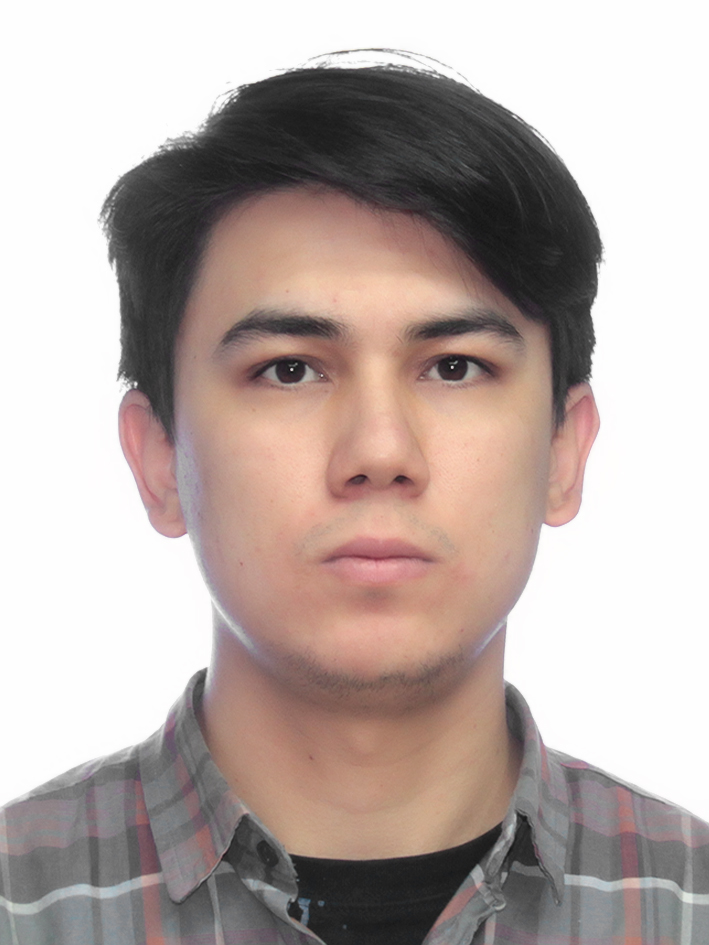
\includegraphics[width=3.5cm]{photo.jpg}
\end{textblock*}

%----------------------------------------------------------------------------------------
%	SUMMARY
%----------------------------------------------------------------------------------------

\begin{rSection}{}
\begin{minipage}[t]{0.83\textwidth}
Computer Vision Engineer with 3+ years of experience in \textbf{3D point cloud processing}, \textbf{sensor calibration}, and \textbf{algorithm optimization}. Currently working on SLAM and LiDAR-based perception for robotics and industrial scanning.
\end{minipage}%
\end{rSection}

%----------------------------------------------------------------------------------------
%	EXPERIENCE
%----------------------------------------------------------------------------------------

\vspace{-0.2cm}
\begin{rSection}{EXPERIENCE}
\vspace{-0.05cm}

\textbf{3D Computer Vision Engineer} \hfill July 2025 - now\\
\textit{{\href{https://vitom-tech.com/en/}{\color{blue}{VITOM Inc.}}}, {SLAM Team} \hfill {Tokyo, Japan}} \\

\vspace{-0.75cm}
\begin{itemize}
    \itemsep -7pt {}
    \item Built the multi-sensor time synchronization layer: PTP across LiDAR, IMU, and camera with hardware/software timestamping, achieving sub-ms camera--LiDAR and $\sim$1 ms IMU--LiDAR precision.
    \item Replaced the production dynamic-object removal system across all scanner models; optimized memory usage for 64 GB machines, enabling processing of up to 3.5 billion points.
    \item Developed a colorization pipeline that projects wide-angle RGB imagery onto SLAM-reconstructed LiDAR maps. 1--2 px projection accuracy at $1920\times1440$.
    \item Rebuilt the scanner web app from legacy PHP to Flask with a modular JS frontend.
    \item Led the port of the SLAM codebase from Python to C++ and the move off Open3D onto in-house geometry.
\end{itemize}

\vspace{-0.15cm}
\textbf{Computer Vision Engineer} \hfill October 2023 - July 2025\\
\textit{{\href{https://kamic.or.kr/en/regional-center/ulsan/}{\color{blue}{Korea Institute of Industrial Technology}}}, 3D Printing Manufacturing Process Center\hfill {Ulsan, South Korea}} \\

\vspace{-0.75cm}
\begin{itemize}
    \itemsep -7pt {}
    \item Built an automated point-cloud inspection pipeline for shipbuilding components covering segmentation, CAD-to-scan registration, and deviation analysis. Delivered the pipeline in joint research with Hyundai Heavy Industries, who built on the algorithms.
    \item Developed an LLM-assisted search platform for 350+ industrial CAD models using natural-language queries and interactive 3D visualization, running on-premise to keep partner data in their environment.
\end{itemize}

\vspace{-0.15cm}
\textbf{Software Engineer} \hfill December 2022 - October 2023\\
\textit{{\href{http://www.klabs.co.kr/en}{\color{blue}{K-Labs}}}, {Software Development Team} \hfill {Ulsan, South Korea}} \\

\vspace{-0.75cm}
\begin{itemize}
    \itemsep -7pt {}
    \item Converted a largely manual scan-to-CAD pipeline to partial automation, cutting operator time per conversion.
    \item Integrated point-cloud post-processing and denoising into internal engineering tools.
\end{itemize}

\end{rSection}

%----------------------------------------------------------------------------------------
%	SKILLS
%----------------------------------------------------------------------------------------

\vspace{-0.3cm}
\begin{rSection}{Skills}
\vspace{-0.05cm}
\textbf{Programming:}{ Python, C++, JavaScript} \\
\textbf{3D Vision \& Point Clouds:}{ Open3D, PCL, OpenCV, PyVista, Trimesh, Three.js, CloudCompare, MeshLab} \\
\textbf{Robotics \& SLAM:}{ SLAM, VSLAM, sensor fusion, LiDAR--IMU--Camera calibration, 3D reconstruction, ROS 2} \\
\textbf{Tools \& Platforms:}{ Linux, Docker, PyTorch} \\
\textbf{Languages:}{ English (advanced), Kazakh (native), Russian (bilingual), Turkish (B2), Korean (TOPIK 2)}
\end{rSection}

%----------------------------------------------------------------------------------------
%	EDUCATION
%----------------------------------------------------------------------------------------

\vspace{-0.3cm}
\begin{rSection}{Education}
\vspace{-0.05cm}

{\bf \href{https://www.timeshighereducation.com/world-university-rankings/university-ulsan}{\color{blue}{University of Ulsan}}} \hfill \textit{Ulsan, South Korea} \\
{Master of Science in AI and Computer Engineering, GPA: 4.1/4.5} \hfill {September 2023 - August 2025} \\
{\it Thesis:} Automated Noise Removal and CAD-to-Scan Comparison for Ship Component Inspection Using Terrestrial LiDAR Scanning \href{https://oak.ulsan.ac.kr/handle/2021.oak/20336}{\faPaperclip} \\
{\bf \href{https://www.timeshighereducation.com/world-university-rankings/nazarbayev-university}{\color{blue}{Nazarbayev University}}} \hfill \textit{Astana, Kazakhstan}\\
{Bachelor of Science in Computer Science, GPA: 3.2/4.0} \hfill {August 2018 - June 2022}
\end{rSection}

%----------------------------------------------------------------------------------------
%	POSTERS AND PRESENTATIONS
%----------------------------------------------------------------------------------------

\vspace{-0.3cm}
\begin{rSection}{Posters and Presentations}
\vspace{-0.05cm}
\begin{itemize}
    \itemsep -7.5pt {}
    \item \underline{\textbf{S.Amangeldi}}, S.B.Park, J.H.Ha, Y.K.Kwon, D.H.Kim "AI-Assisted Search for Industrial Components Using a Local Database and Large Language Models", International Conference on Precision Engineering and Sustainable Manufacturing 2025 (PRESM2025), Chiang Mai, Thailand, July 2025
    \textbf{(poster)}

    \item \underline{\textbf{S.Amangeldi}}, N.T.Phan, A.Tleuliyev, Y.K.Kwon, D.H.Kim "Comparative Analysis of Point Cloud Scans and 3D CAD Data for Dimensional Inspection in Shipbuilding Components", Korean Society for Precision Engineering Conference (KSPE), Jeju, South Korea, May 2024
    \href{https://www.dbpia.co.kr/journal/articleDetail?nodeId=NODE11798461}{\faPaperclip} \textbf{(poster)}

    \item Co-author on three further KSPE 2024 papers, on additive manufacturing for shipbuilding production, supplier selection via genetic algorithms, and audio representations synthesized from 3D models.
\end{itemize}

\end{rSection}

\end{document}
